% \documentclass{beamer}
 \documentclass[handout]{beamer}

\usetheme{default}

\usepackage[english]{babel}
\usepackage[latin1]{inputenc}

\usepackage{times}
\usepackage[T1]{fontenc}

%%
%%  some useful macro definitions & configuration settings
%%

\usepackage{latexsym}
\usepackage{graphicx}
\usepackage{url}
\usepackage{alltt}              % code examples with nicely formatted comments
\usepackage{xcolor}
\usepackage{pifont}
\usepackage{xspace}
\usepackage{array,booktabs}

\definecolor{quietred}{rgb}{.6,.2,.1}
\definecolor{quietblue}{rgb}{.1,.2,.7}
\definecolor{brightred}{rgb}{.9,0,.1}

%% > plot(x,y)      \REM{this produces a scatterplot}
\newcommand{\REM}[1]{\textsf{\small\color{quietred}\# #1}}

%% nice colour for R output: \begin{Rout} .. \end{Rout}
\newenvironment{Rout}{%
  \begin{footnotesize}\color{quietblue}\bfseries}{%
  \color{black}\mdseries\end{footnotesize}}

%% ... This is something \h{important}. ...
\newcommand<>{\h}[1]{\textbf#2{\color#2{quietred}#1}}
\newcommand<>{\hh}[1]{\textbf#2{\color#2{brightred}#1}}

%% cite \textcite{some text} in roman italic font
\newcommand{\textcite}[1]{\textrm{\textit{#1}}}

%% how can you live without the arrow (\so) and the hand (\hand) ?
\newcommand{\so}{\ding{234}\xspace}
\newcommand{\So}{\hh{\ding{229}}\xspace}
\newcommand{\hand}{\ding{43}\xspace}

%% \p{X=k};  \pC{X=k}{Y=l};  \bigp{X_i = k};   \pscale{\frac{Z}{S^2}};
%% probability P(X=k) and conditional probability P(X=k|Y=l), also with larger or scaled parentheses
%% \p[\theta]{X=k};  \pC[\text{interpolated}]{X=k}{Y=l};  ...
%% with optional subscripts (for model probability, null probability, etc.)
\newcommand{\p}[2][]{\mathop{\text{Pr}_{#1}}(#2)}
\newcommand{\pscale}[2][]{\mathop{\text{Pr}_{#1}}\!\left(#2\right)}
\newcommand{\bigp}[2][]{\mathop{\text{Pr}_{#1}}\bigl(#2\bigr)}
\newcommand{\pC}[3][]{\p[#1]{#2\,|\,#3}} 
\newcommand{\pCscale}[3][]{\pscale[#1]{#2\left|\,#3\right.\!}} 
\newcommand{\bigpC}[3][]{\bigp[#1]{#2\bigm|#3}} 

%% \Exp{X};  \Var{X};  \Exp[0]{X};  \Var[0]{X};  
%% \bigExp{X}; \bigVar{X}; \Expscale{X};  \Varscale{X};
%% expectation E[X] and variance V[X], expectation and variance under null hypothesis, 
%% and variants with largeer or scaled brackets
\newcommand{\Exp}[2][]{\text{E}_{#1}[#2]}
\newcommand{\Var}[2][]{\mathop{\text{Var}}_{#1}[#2]}
\newcommand{\bigExp}[2][]{\text{E}_{#1}\!\bigl[#2\bigr]}
\newcommand{\bigVar}[2][]{\mathop{\text{Var}}_{#1}\bigl[#2\bigr]}
\newcommand{\Expscale}[2][]{\text{E}_{#1}\left[#2\right]}
\newcommand{\Varscale}[2][]{\mathop{\text{Var}}_{#1}\left[#2\right]}


\title[SIGIL: NN Compounds]{Statistical Analysis of Corpus Data with R}
\subtitle{Distributional properties of Italian NN compounds:\\
  An Exploration with R}

\author[Baroni \& Evert]{Designed by Marco Baroni\inst{1} and Stefan Evert\inst{2}}
\institute{
  \inst{1}Center for Mind/Brain Sciences (CIMeC)\\
  University of Trento
  \and
  \inst{2}Institute of Cognitive Science (IKW)\\
  University of Onsabr�ck
}
\date{}


\begin{document}

\frame{\titlepage}


\begin{frame}
  \frametitle{Outline}
  \tableofcontents
\end{frame}

\section{Introduction}

\begin{frame}
  \frametitle{NN Compounds}

  \begin{itemize}
  \item Part of work carried out by Marco Baroni with Emiliano Guevara
    (U Bologna) and Vito Pirrelli (CNR/ILC, Pisa)
  \item Three-way classification inspired by theoretical (Bisetto and
    Scalise, 2005) and psychological work (e.g., Costello and Keane,
    2001)
    \begin{itemize}
    \item \h{Relational} (\emph{computer center}, \emph{angolo bambini})
    \item \h{Attributive} (\emph{swordfish}, \emph{esperimento pilota})
    \item \h{Coordinative} (\emph{singer-songwriter}, \emph{bar pasticceria})
    \end{itemize}
  \end{itemize}
\end{frame}

\begin{frame}
  \frametitle{Relational compounds}

  \begin{itemize}
  \item Express relation between two entities
  \item Heads are typically information containers, organizations,
    places, aggregators, pointers, etc.
  \item \textbf{M} ``grounds'' generic meaning of, or fills slot of
    \textbf{H}
  \item E.g., \emph{stanza server} (``server room''), \emph{fondo
      pensioni} (``pension fund''), \emph{centro citt�} (``city
    center'')
    \end{itemize}


\end{frame}


\begin{frame}
  \frametitle{Attributive compounds}

  \begin{itemize}
  \item Interpretation of \textbf{M} is reduced to a ``salient''
    property of its full semantic content, and this property is
    \emph{attributed} to \textbf{H}:
  \item \emph{presidente fantoccio} (``puppet president''),
    \emph{progetto pilota} (``pilot project'')
  \end{itemize}
\end{frame}

\begin{frame}
  \frametitle{Coordinative compounds}
  \begin{itemize}
  \item Head and modifier denote similar/compatible entities, compound
    has coordinative reading
  \item \textbf{HM} is both \textbf{H} and \textbf{M}
  \item \emph{viaggio spedizione} (``expedition travel''),
    \emph{cantante attore} (``singer actor'')
  \item Ignored here
  \end{itemize}
\end{frame}


\begin{frame}
  \frametitle{Ongoing exploration}

  \begin{itemize}
  \item Data-set of frequent compounds: 24 \textbf{ATT} / 100 \textbf{REL}
  \item All \textbf{ATT} and \textbf{REL} compounds with freq $\geq
    1,000$ in itWaC (2 billion token Italian Web-based corpus)
  \item Will the distinction between \textbf{ATT} and \textbf{REL}
    emerge from combination of distributional cues (also extracted
    from itWaC)?  \pause
  \item Cues:
    \begin{itemize}
    \item Semantic similarity between head and modifier
    \item Explicit syntactic link
    \item Relational properties of head and modifier
    \item ``Specialization'' of head and modifier
    \end{itemize}
  \end{itemize}

\end{frame}


\AtBeginSection[]
{
  \begin{frame}
    \frametitle{Outline}
    \tableofcontents[current,currentsection]
  \end{frame}
}


\AtBeginSubsection[]
{
  \begin{frame}
    \frametitle{Outline}
    \tableofcontents[current,currentsubsection]
  \end{frame}
}

\section{Data}


\begin{frame}
  \frametitle{The data}

    \begin{description}
    \item[H] Compound head (Italian compounds are left-headed!)
    \item[M] Modifier
    \item[TYPE] \alert{at}tributive or \alert{re}lational
    \item[COS] Cosine similarity between \textbf{H} and \textbf{M}
    \item[DELLL] Log-likelihood ratio score for comparison between
      observed frequency of \emph{\textbf{H} del \textbf{M}} (``\textbf{H} of the \textbf{M}'') and
      expected frequency under independence
    \item[HDELPROP] Proportion of times \textbf{H} occurs in context \emph{\textbf{H}
        del NOUN} over total occurrences of \textbf{H}
    \item[DELMPROP] Proportion of times \textbf{M} occurs in context \emph{NOUN
        DEL M} over total occurrences of \textbf{M}
    \item[HNPROP] Proportion of times \textbf{H} occurs in context \emph{H
        NOUN} over total occurrences of \textbf{H}
    \item[NMPROP] Proportion of times \textbf{M} occurs in context \emph{NOUN
        M} over total occurrences of \textbf{M}
    \end{description}

\end{frame}


\begin{frame}
  \frametitle{Cue statistics}

  \begin{itemize}
  \item Read the file \texttt{comp.stats.txt} into a data-frame named
    \texttt{d} and ``attach'' the data-frame
    \begin{itemize}
    \item[\hand] load file with \texttt{read.delim()} function as recommended
    \item[\hand] use option \texttt{encoding="UTF-8"} on Windows
    \end{itemize}
  \item Compute basic statistics
  \item Look at the distribution of each cue among compounds of type
    attributive (\texttt{at}) vs.~relational (\texttt{re})
  \item Find out for which cues the distinction between attributive and
    relational is significant (using a $t$-test or Mann-Whitney ranks test)
  \item Also, which cues are correlated? (use \texttt{cor()} on the
    subset of the data-frame that contains the cues)
  \end{itemize}

\end{frame}

\section{Clustering}

\subsection{$k$-means}

\begin{frame}
  \frametitle{Clustering}

  \begin{itemize}
  \item \emph{k-means}: one of the simplest and most widely used hard flat
    clustering algorithms
  \item For more sophisticated options, see the \emph{cluster} and
    \emph{e1071 }packages
  \end{itemize}

\end{frame}

\begin{frame}
  \frametitle{k-means}
  \begin{itemize}
  \item The basic algorithm
    \begin{enumerate}
    \item Start from $k$ random points as cluster centers
    \item Assign points in data-set to cluster of closest center
    \item Re-compute centers (means) from points in each cluster
    \item Iterate cluster assignment and center update steps until
      configuration converges
    \end{enumerate}
  \item Given random nature of initialization, it pays off to repeat
    procedure multiple times (or to start from ``reasonable''
    initialization)
  \end{itemize}
\end{frame}


\begin{frame}
  \frametitle{Illustration of the $k$-means algorithm}
  \framesubtitle{See \texttt{help(iris)} for more information about the data
    set used}

  \begin{center}
    \includegraphics[width=80mm]<beamer:1| handout:0>{img/clustering-iris-kmeans-1a}%
    \includegraphics[width=80mm]<beamer:2| handout:1>{img/clustering-iris-kmeans-1b}%
    \includegraphics[width=80mm]<beamer:3| handout:0>{img/clustering-iris-kmeans-1c}%
    \includegraphics[width=80mm]<beamer:4| handout:2>{img/clustering-iris-kmeans-2a}%
    \includegraphics[width=80mm]<beamer:5| handout:0>{img/clustering-iris-kmeans-2b}%
    \includegraphics[width=80mm]<beamer:6| handout:3>{img/clustering-iris-kmeans-3a}%
    \includegraphics[width=80mm]<beamer:7| handout:0>{img/clustering-iris-kmeans-3b}%
    \includegraphics[width=80mm]<beamer:8| handout:0>{img/clustering-iris-kmeans-4a}%
    \includegraphics[width=80mm]<beamer:9| handout:0>{img/clustering-iris-kmeans-4b}%
    \includegraphics[width=80mm]<beamer:10| handout:0>{img/clustering-iris-kmeans-5a}%
    \includegraphics[width=80mm]<beamer:11| handout:0>{img/clustering-iris-kmeans-5b}%
  \end{center}
\end{frame}



\begin{frame}[fragile]
  \frametitle{\emph{k}-means, first try}

 \begin{alltt}
\REM{cues are in columns 4 to 9}

> km <- kmeans(d[,4:9], 2, nstart=10)
> km

\REM{problem: extreme DELLL values dominate the clustering}
\REM{(relevant small cluster might be cluster 2 in your solution)}

> DELLL[km\$cluster==1]

> head(sort(DELLL, decreasing=TRUE))
\end{alltt}
\end{frame}


\begin{frame}[fragile]
  \frametitle{Scaling and trying again}

\begin{alltt}
> scaled <- scale(d[,4:9])
> summary(d[4:9])  \REM{distribution of original data}
> summary(scaled)  \REM{after scaling}

> km <- kmeans(scaled, 2, nstart=10)
> km

> table(km\$cluster, d\$TYPE) \REM{confusion matrix}
\end{alltt}

\end{frame}

\subsection{Dimenstionality reduction with PCA}

\begin{frame}
  \frametitle{Dimensionality reduction}

  \begin{itemize}
  \item To find ``latent'' variables
  \item To reduce random noise
  \item For easier visualization
  \end{itemize}

\end{frame}


\begin{frame}
  \frametitle{Principal component analysis (PCA)}

  \begin{itemize}
  \item Find a set of orthogonal dimensions such that the first
    dimension ``accounts'' for the most \emph{variance} in the original
    data-set, the second dimension accounts for as much as possible of
    the remaining variance, etc.
  \item The top $k$ dimensions (principal components) are the best
    sub-set of $k$ dimensions to approximate the spread in the
    original data-set
  \item Principal components represent correlations of original variables \so
    might reveal interesting underlying patterns
  \end{itemize}
\end{frame}


\begin{frame}
  \frametitle{Preserving variance: examples}

  \begin{center}
    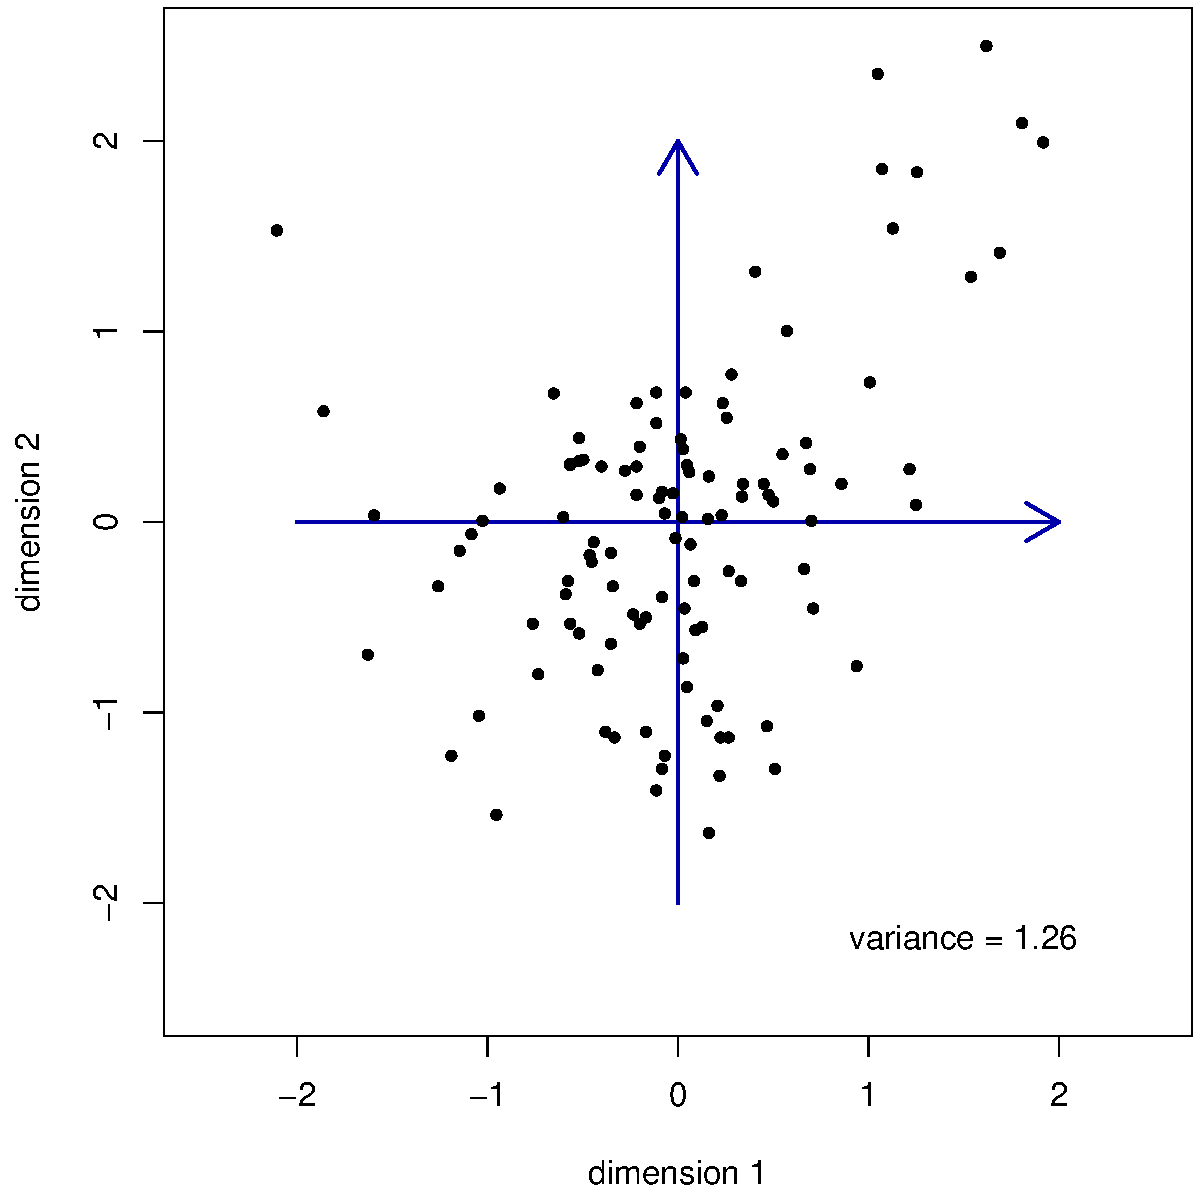
\includegraphics[width=7cm]{img/pca_variance}%
  \end{center}
\end{frame}


\begin{frame}<beamer:1-6| handout:1-3>[c]
  \frametitle{Preserving variance: examples}

  \begin{center}
    \only<beamer:1| handout:0>{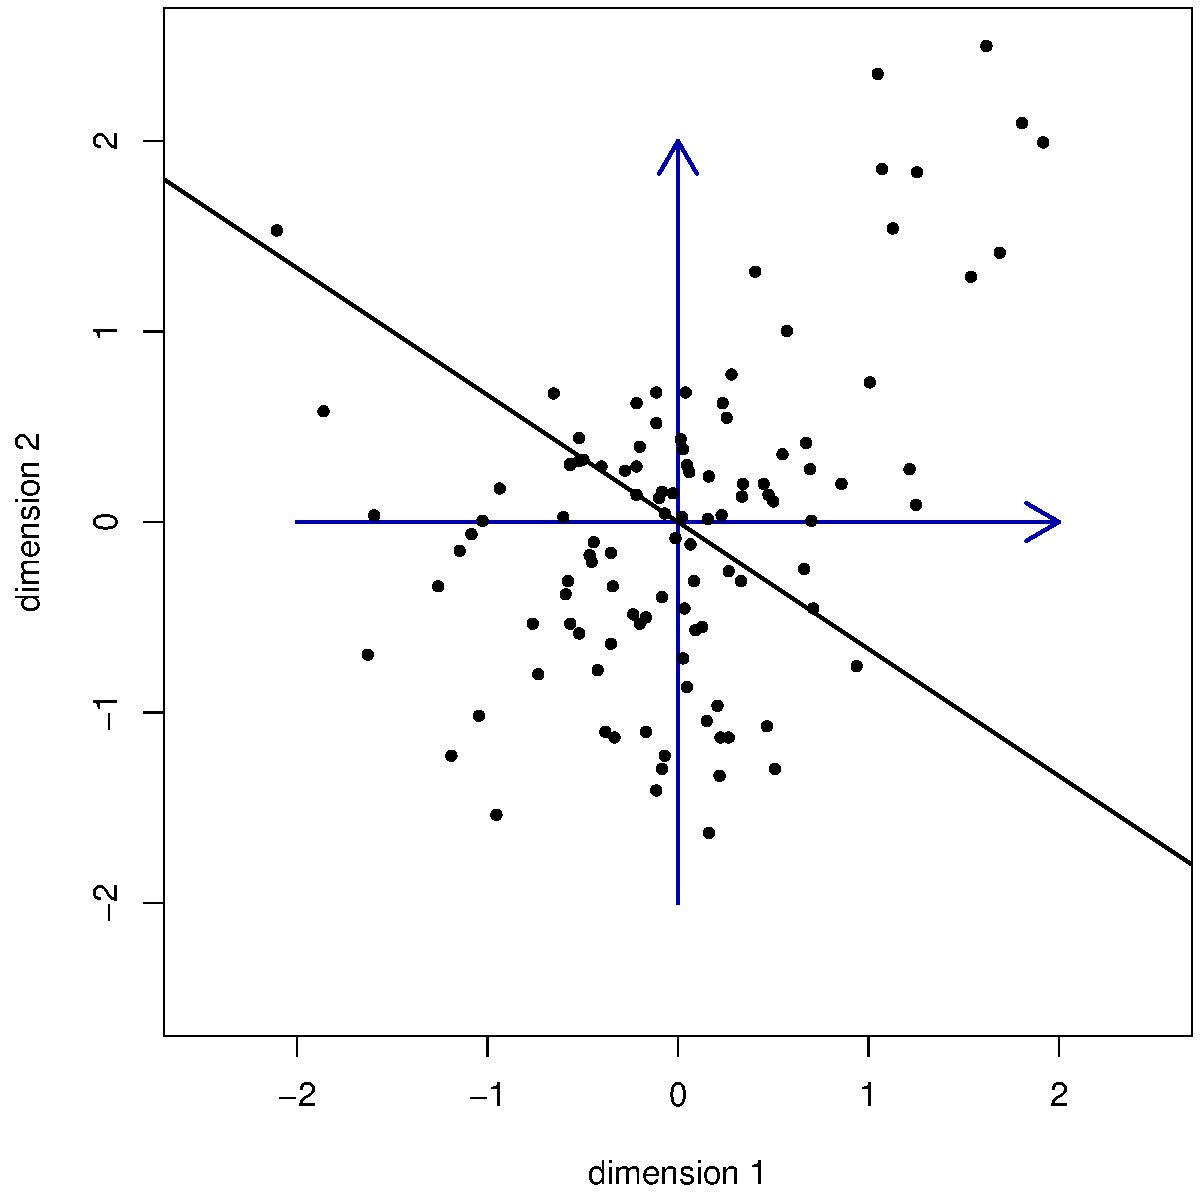
\includegraphics[width=7cm]{img/pca_1_axis}}%
    \only<beamer:2| handout:1>{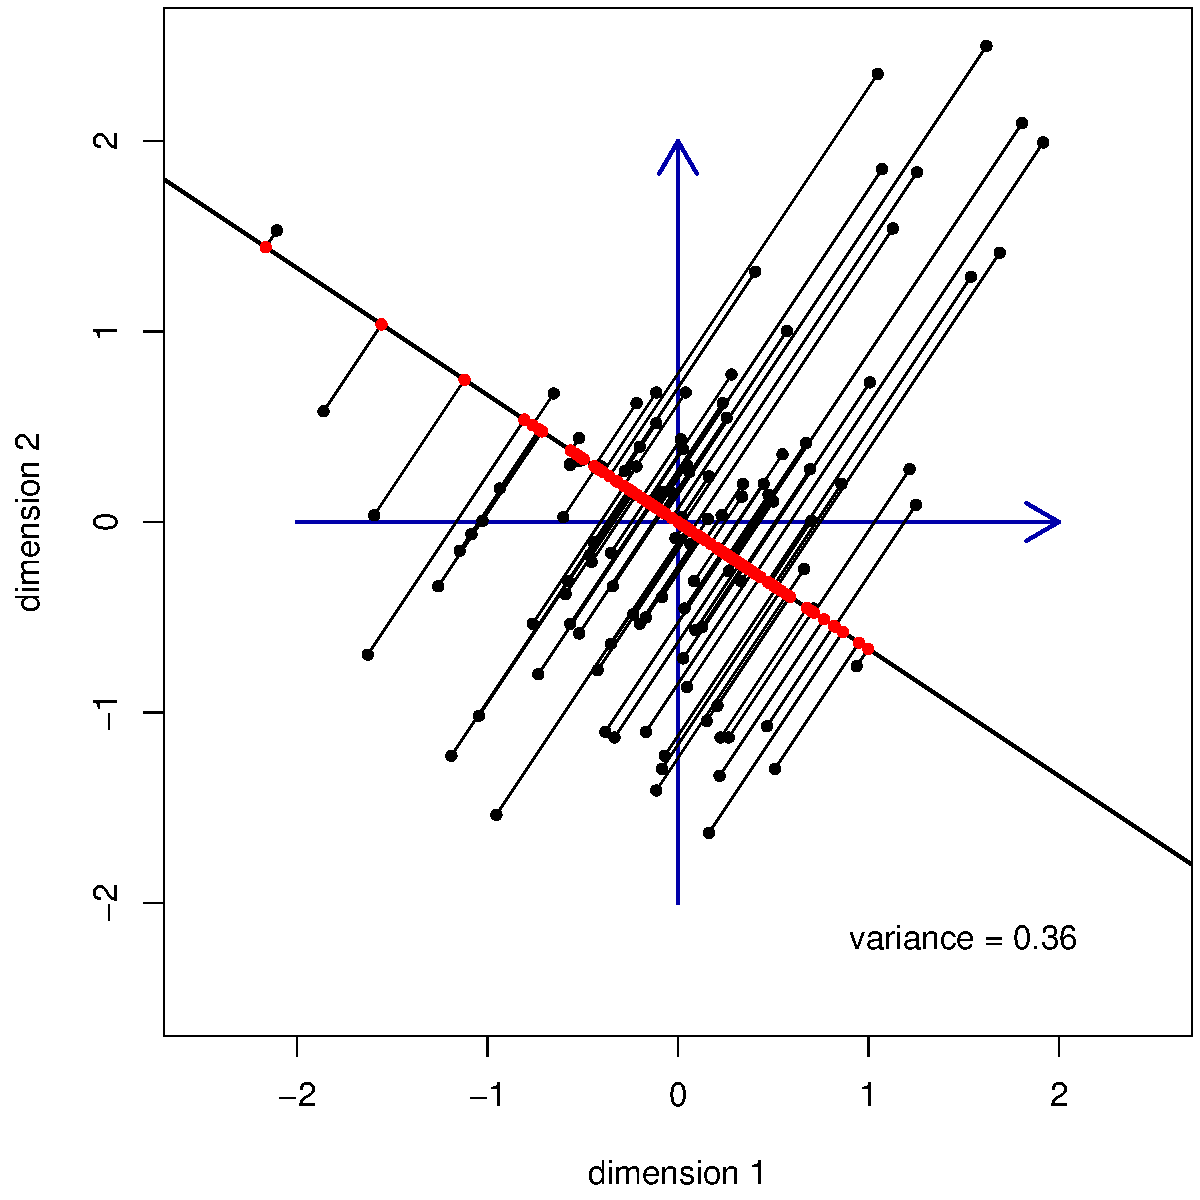
\includegraphics[width=7cm]{img/pca_1_projection}}%
    \only<beamer:3| handout:0>{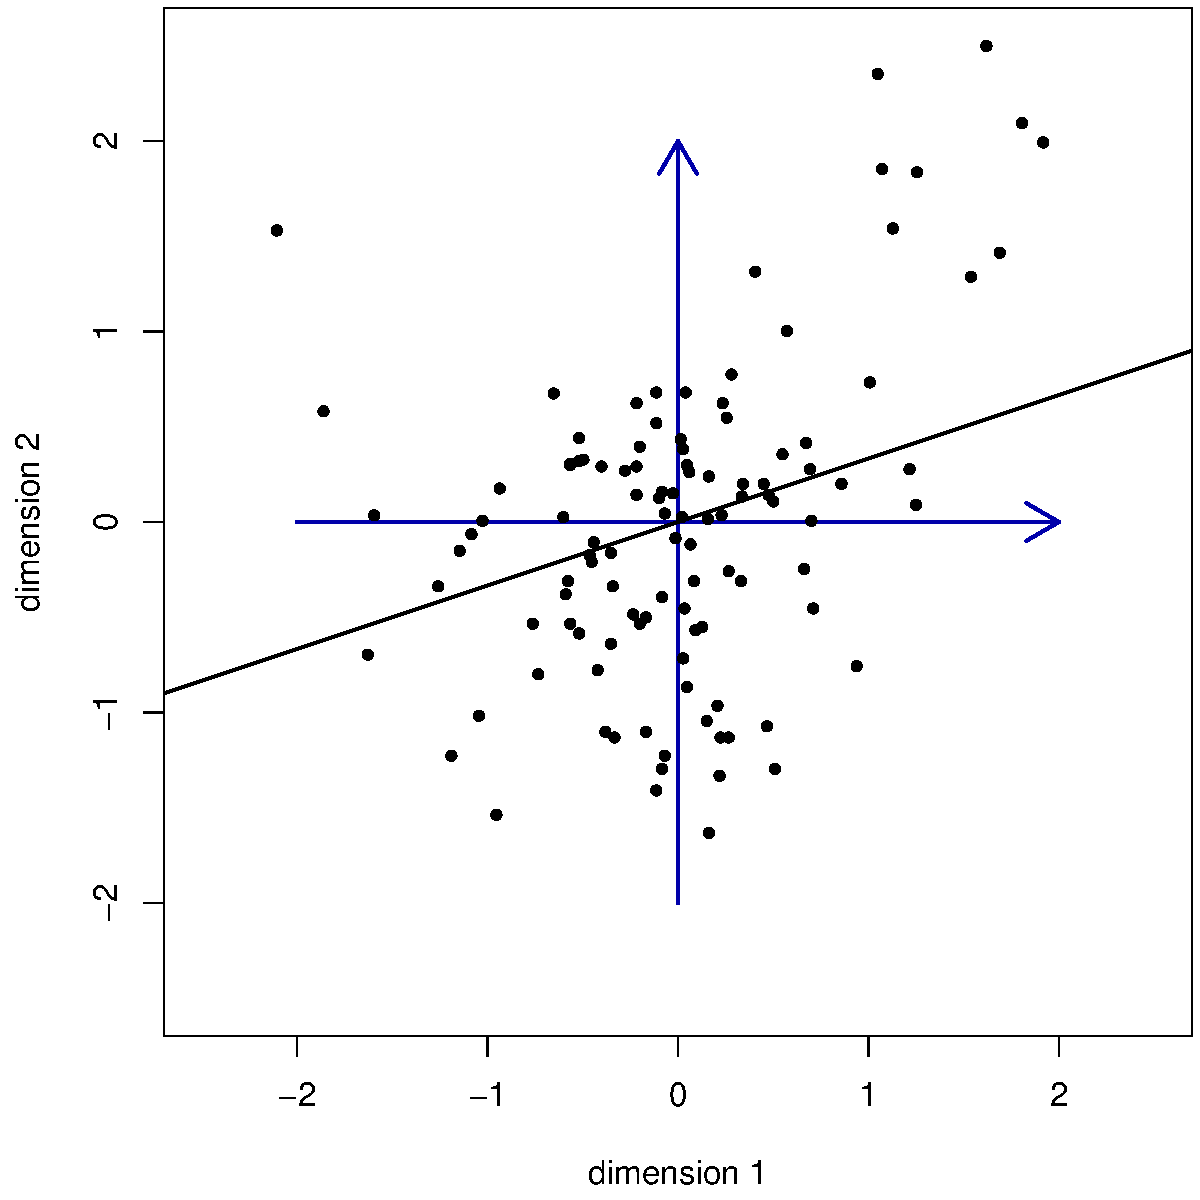
\includegraphics[width=7cm]{img/pca_2_axis}}%
    \only<beamer:4| handout:2>{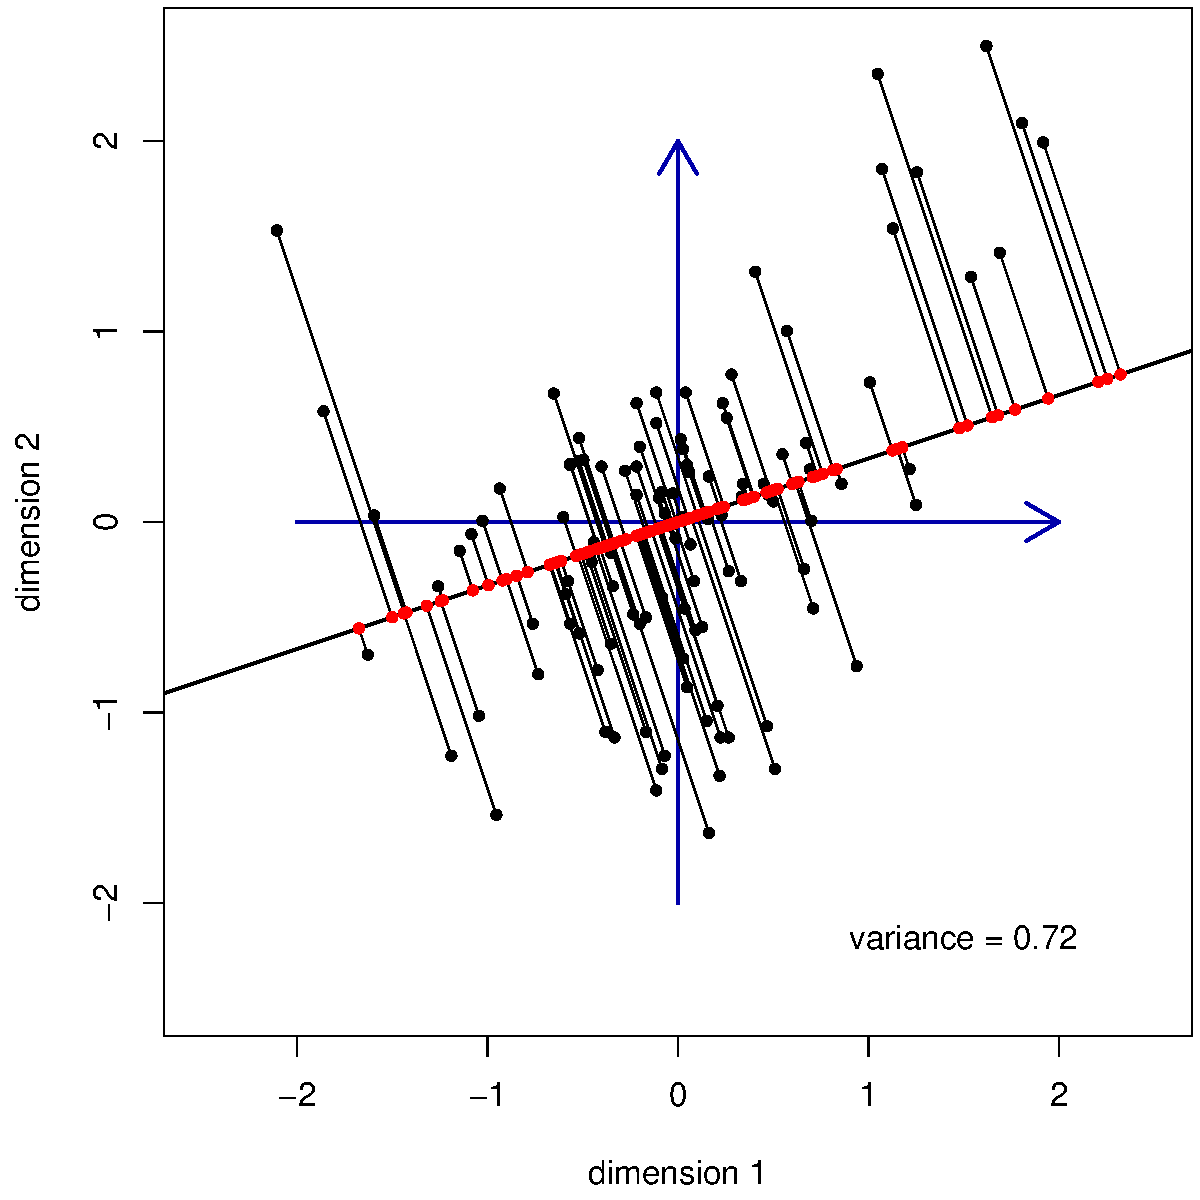
\includegraphics[width=7cm]{img/pca_2_projection}}%
    \only<beamer:5| handout:0>{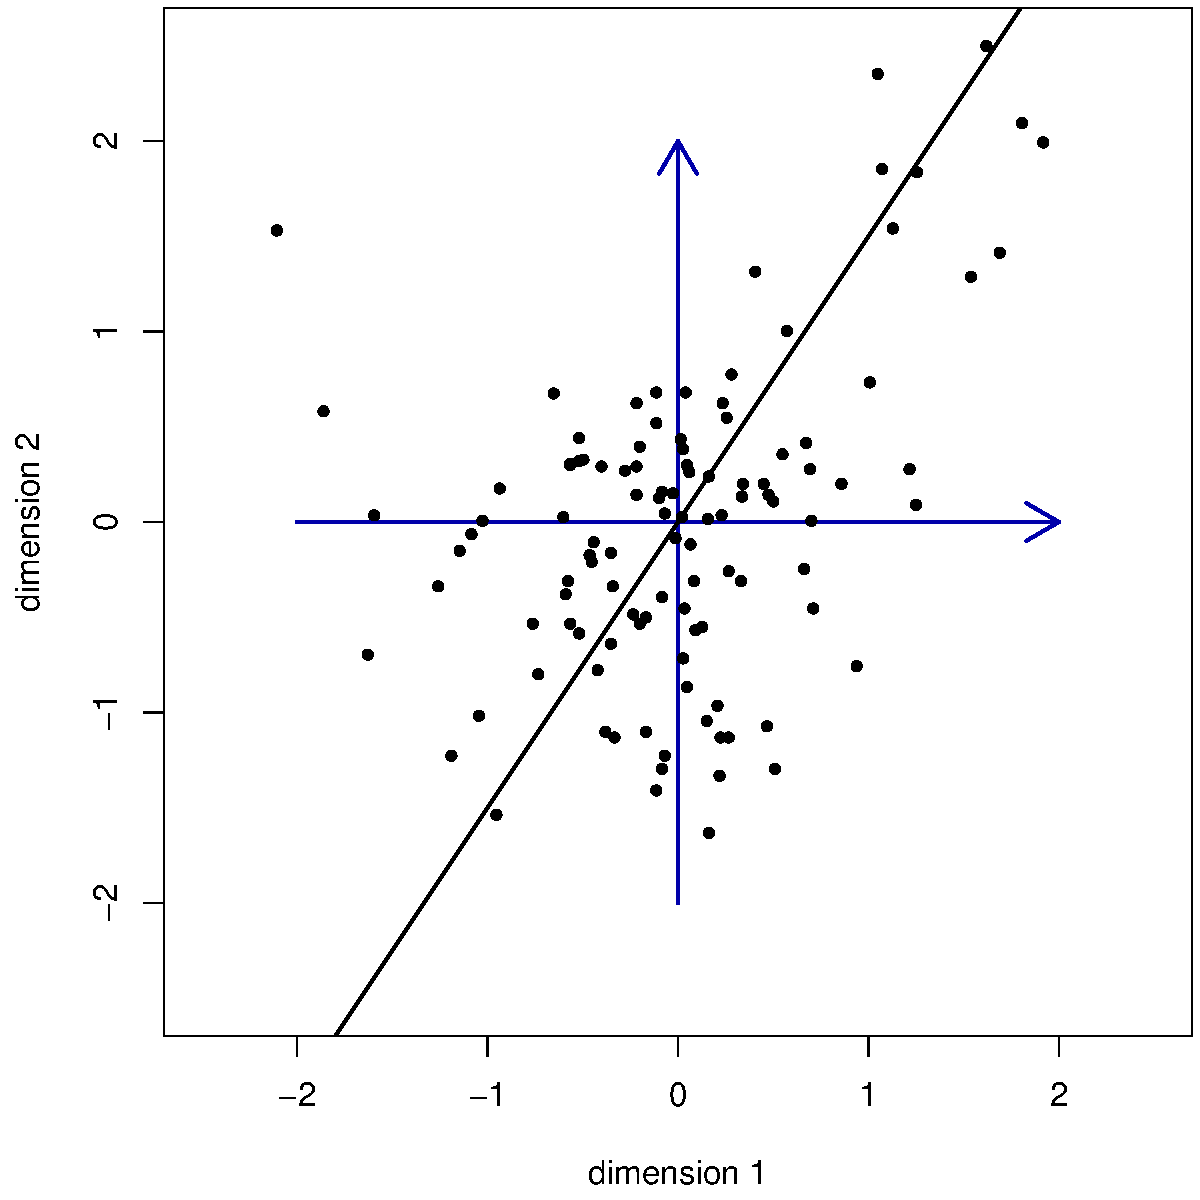
\includegraphics[width=7cm]{img/pca_3_axis}}%
    \only<beamer:6| handout:3>{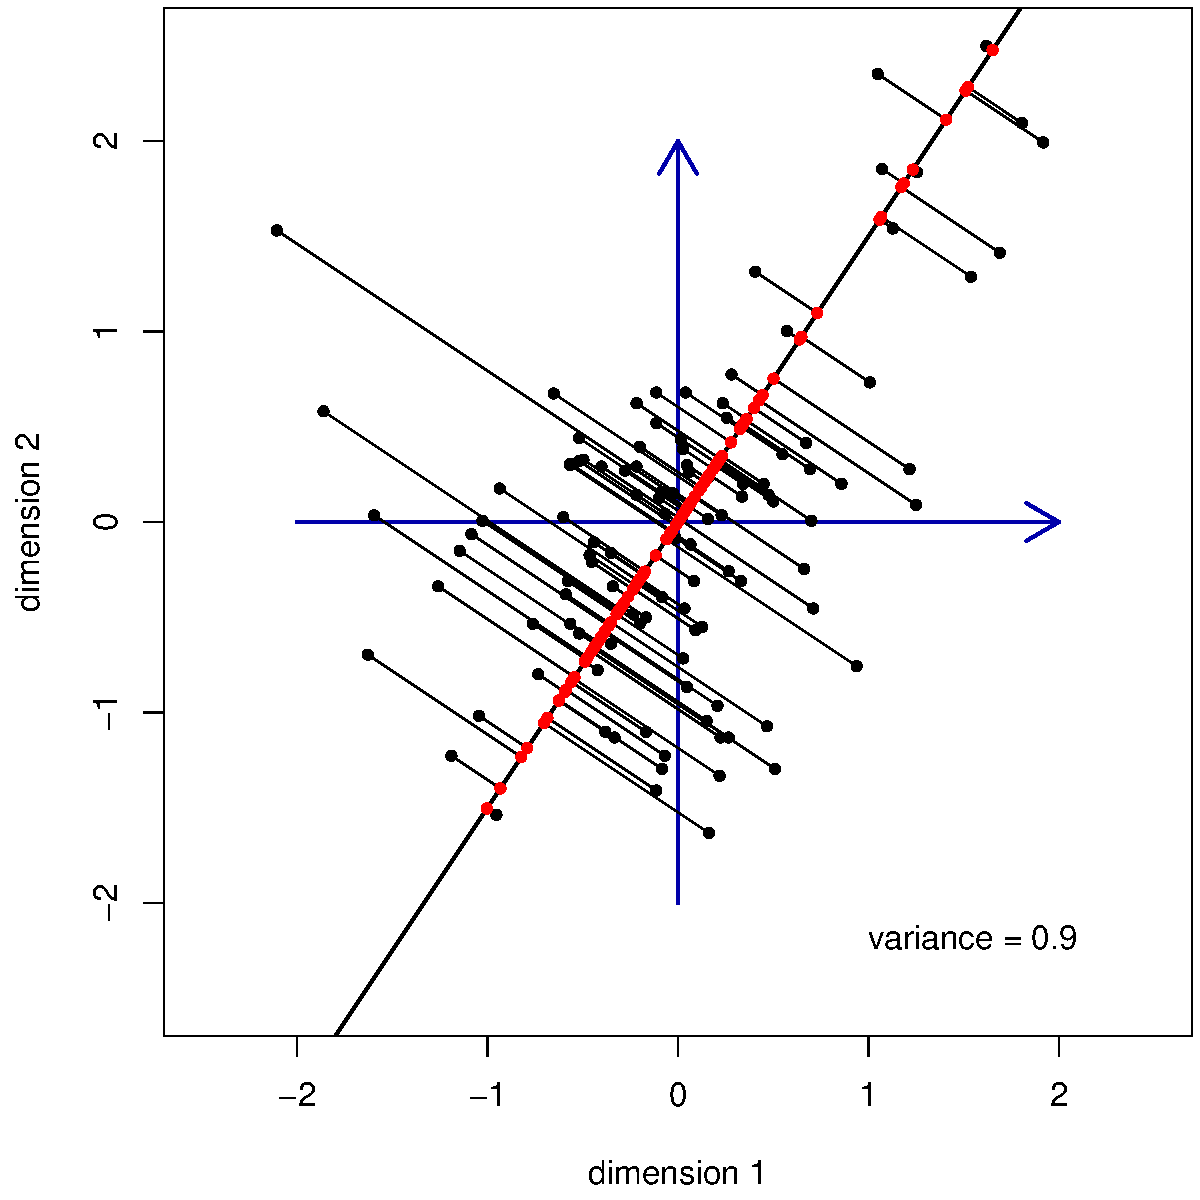
\includegraphics[width=7cm]{img/pca_3_projection}}%
  \end{center}
\end{frame}


\begin{frame}
  \frametitle{Adding an orthogonal dimension}

  \begin{center}
    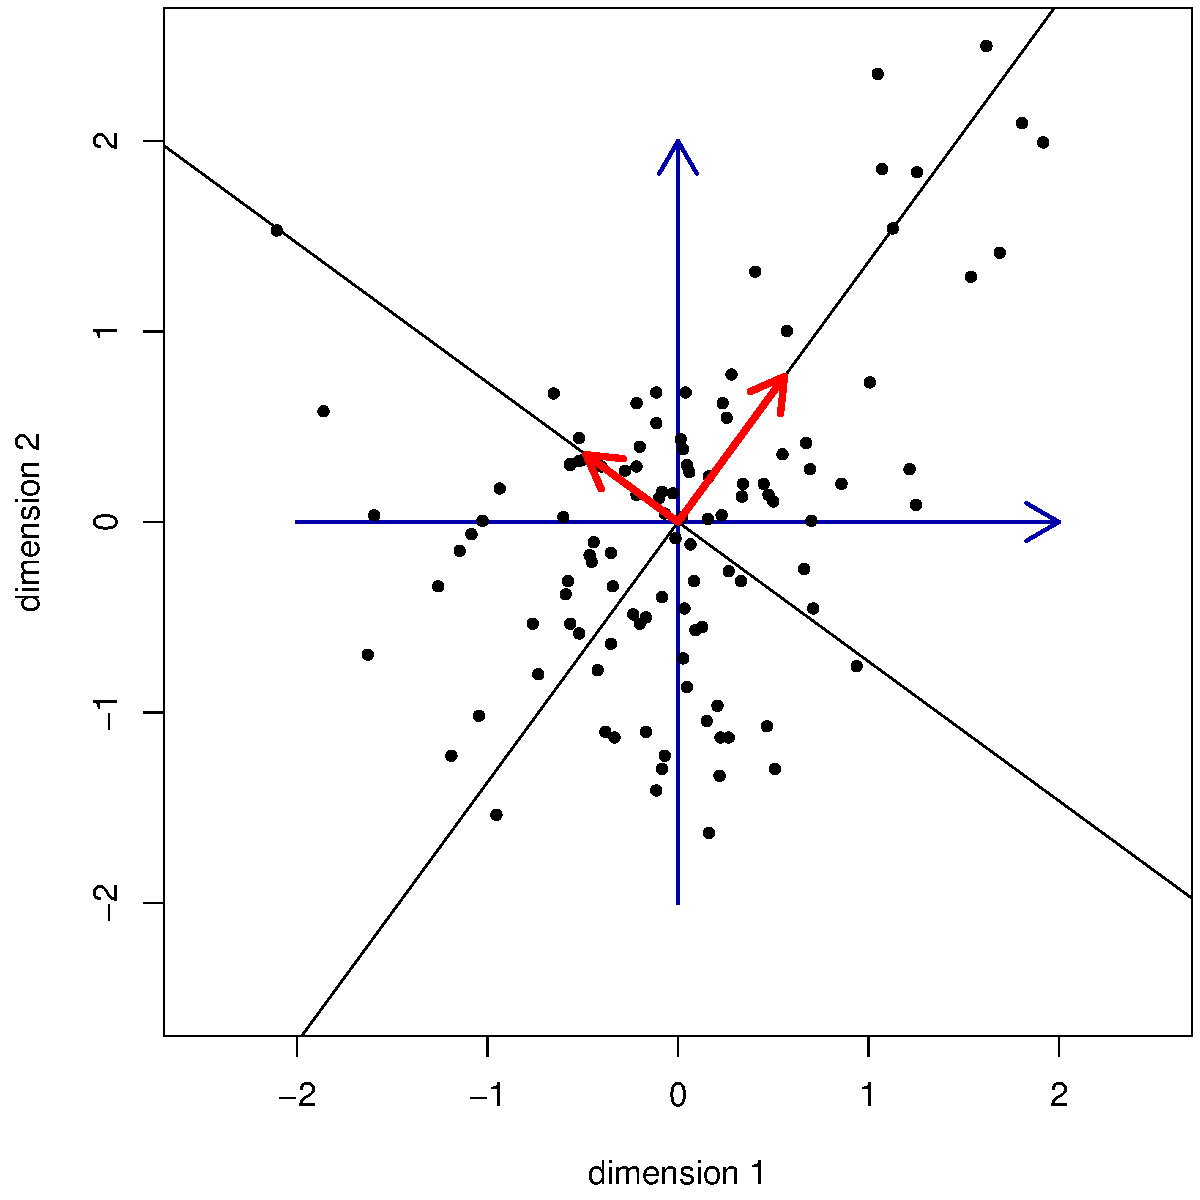
\includegraphics[width=7cm]{img/pca_pca}%
  \end{center}
\end{frame}

\begin{frame}[fragile]
  \frametitle{PCA in R}
  \begin{verbatim}
> temp <- subset(d, select=c(HNPROP, NMPROP,
  DELLL, HDELPROP, DELMPROP, COS))

> pr <- prcomp(temp, scale=TRUE)
> pr

> plot(pr)

> biplot(pr)
> biplot(pr, xlabs=TYPE, 
  xlim=c(-.25,.25), ylim=c(-.25,.25))
\end{verbatim}
\end{frame}

\begin{frame}[fragile]
  \frametitle{More refined plotting}
  \begin{alltt}
> plot(pr\$x[,1:2], type="n", 
  xlim=c(min(pr\$x[,1]),4),
  ylim=c(min(pr\$x[,2]),4))   \REM{only sets up plot region}

> points(subset(pr\$x, TYPE=="re"), 
  col="blue", pch=19, lwd=2) \REM{blue points for type ``re''}

> points(subset(pr\$x, TYPE=="at"), 
  col="red", pch=19, lwd=2)  \REM{red points for type ``at''}

> legend("topright", inset=.05, 
  fill=c("red","blue"), cex=1.5,
  legend=c("ATT","REL"))     \REM{legend explains colors}
\end{alltt}
\end{frame}

\begin{frame}[fragile]
  \frametitle{Adding the cues}

  \begin{alltt}
> text(pr\$rotation[1,1]*4, pr\$rotation[1,2]*4,
  label="H N", cex=1.7)

> text(pr\$rotation[2,1]*4, pr\$rotation[2,2]*4,
  label="N M", cex=1.7)

> text(pr\$rotation[3,1]*4, pr\$rotation[3,2]*4,
  label="H DEL M", cex=1.7)

> text(pr\$rotation[4,1]*4, pr\$rotation[4,2]*4,
  label="H DEL", cex=1.7)

> text(pr\$rotation[5,1]*4, pr\$rotation[5,2]*4,
  label="DEL M", cex=1.7)

> text(pr\$rotation[6,1]*4, pr\$rotation[6,2]*4,
  label="COS", cex=1.7)
\end{alltt}
\end{frame}

\begin{frame}[fragile]
  \frametitle{Trying k-means again}
  \begin{alltt}
> km <- kmeans(pr\$x[,1:4], 2, nstart=10)
> table(km\$cluster, d\$TYPE)    

\REM{what happens with more/fewer dimensions?}

> plot(pr\$x[,1:2], type="n",
  xlim=c(min(pr\$x[,1]),4),
  ylim=c(min(pr\$x[,2]),4))

> text(pr\$x[,1], pr\$x[,2],
  col=km\$cluster, labels=TYPE)
\REM{now refine this plot as on previous slides}
\end{alltt}
\end{frame}

% \begin{frame}[fragile]
%   \frametitle{Appendix: Multi-Dimensional Scaling}
%   \begin{alltt}
% mds<-cmdscale(dist(scaled))
% plot(mds,type="n")
% points(mds[TYPE=="re",],col="blue")
% points(mds[TYPE=="at",],col="red")

% \REM{see also sammon, isoMDS in the
% # MASS package}
%   \end{alltt}
% \end{frame}

\end{document}
